% =====================================================================
\chapter{Campo Minado: regras do jogo e técnicas de implementação}\label{cap:14}
\naaula{48}

A atividade prática desta aula é um Campo Minado completo, que usa as estruturas das Aulas 1 a 3
e as análises da Aula 4. Este capítulo explica as regras do jogo em detalhes e cada técnica usada
na solução de exemplo (pasta \codigo{solucoes/campo_minado/} do repositório). Os trechos de
código são da solução real; o enunciado da atividade diz o que você deve implementar.

\section{As regras do jogo}

\subsection{O tabuleiro}

O jogo acontece num tabuleiro de $L$ linhas e $C$ colunas de \textbf{células}. Algumas células —
$k$ delas — escondem uma \textbf{mina}. No começo, todas estão \textbf{fechadas}: o jogador não
sabe onde estão as minas. O objetivo é \textbf{abrir todas as células que não têm mina}.

\begin{center}
\begin{tabularx}{0.8\textwidth}{L C C C}
\cab \tc{Nível} & \tc{Linhas × colunas} & \tc{Células} & \tc{Minas} \\
Fácil & $9 \times 9$ & 81 & 10 \\
\rowcolor{edfundo} Médio & $16 \times 16$ & 256 & 40 \\
Difícil & $16 \times 30$ & 480 & 99 \\
\end{tabularx}
\end{center}

\subsection{Os números}

Ao abrir uma célula sem mina, ela mostra um \textbf{número}: quantas minas existem entre as suas
\textbf{vizinhas} — as até 8 células que encostam nela, inclusive nas diagonais. Uma célula no
meio do tabuleiro tem 8 vizinhas; numa borda, 5; num canto, 3. Os números são as pistas do jogo:
um 1 cercado de células abertas, com uma única vizinha fechada, garante que essa vizinha é mina.

\begin{figure}[!htb]
\centering
\begin{tikzpicture}[scale=0.62]
  \fill[edfundo] (0,0) rectangle (5,5);
  \draw[edcinzaclaro, line width=0.8pt] (0,0) grid (5,5);
  \draw[edverde, line width=1.2pt] (0,0) rectangle (5,5);
  \foreach \i in {1,...,5} {
    \node[font=\small\bfseries, color=edverde] at (\i-0.5, 5.4) {\i};
    \node[font=\small\bfseries, color=edverde] at (-0.4, 5.5-\i) {\i};
  }
  \foreach \c/\l in {1/1, 2/1, 5/1, 1/2, 4/2, 5/2, 1/3, 2/3, 3/3, 4/3, 5/3, 4/4, 4/5, 5/5}
    \node[font=\bfseries, color=edteal] at (\c-0.5, 5.5-\l) {1};
  \foreach \c/\l in {3/1, 3/2}
    \node[font=\bfseries, color=edlaranja] at (\c-0.5, 5.5-\l) {2};
  \foreach \c/\l in {1/4, 2/4, 3/4, 1/5, 2/5, 3/5}
    \node[font=\bfseries, color=edcinza] at (\c-0.5, 5.5-\l) {0};
  \foreach \c/\l in {4/1, 2/2, 5/4} {
    \fill[edtexto] (\c-0.5, 5.5-\l) circle (0.2);
    \foreach \a in {0,45,90,135} \draw[edtexto, line width=1pt] ($(\c-0.5, 5.5-\l)+(\a:0.32)$) -- ($(\c-0.5, 5.5-\l)+(\a+180:0.32)$);
  }
\end{tikzpicture}
\caption{O tabuleiro 5 × 5 da atividade (Parte A), com minas em (1,\,4), (2,\,2) e (4,\,5) e os
números de todas as células seguras.}
\end{figure}

\subsection{A abertura em cascata}

Uma célula com \textbf{0} não tem nenhuma mina em volta. Então todas as suas vizinhas são
seguras, e o jogo as abre automaticamente. Se alguma delas também for 0, as vizinhas dela também
se abrem, e assim por diante: uma única jogada pode abrir uma área grande. As células numeradas
formam a \enquote{borda} da área aberta: elas se abrem, mas não espalham a abertura.

\subsection{Bandeiras, primeiro clique, vitória e derrota}

\begin{itemize}
  \item \textbf{Bandeira:} o jogador pode marcar uma célula fechada onde acha que há mina. A
        célula marcada não pode ser aberta (nem pela cascata) até a bandeira ser retirada. O placar
        mostra \enquote{minas menos bandeiras}; ele fica negativo se houver bandeiras demais.
  \item \textbf{Primeiro clique seguro:} as minas só são sorteadas depois do primeiro clique,
        longe da célula clicada e das suas vizinhas. Assim, o primeiro clique sempre abre uma área.
  \item \textbf{Derrota:} abrir uma célula com mina. O jogo mostra todas as minas e marca as
        bandeiras colocadas em lugares errados.
  \item \textbf{Vitória:} abrir todas as células seguras. As minas que faltavam ganham bandeira.
  \item \textbf{Desfazer:} só a última bandeira pode ser desfeita. Abrir uma célula não tem volta.
\end{itemize}

\subsection{Como jogar nas duas interfaces}

Na \textbf{interface gráfica} (\codigo{jogo_gui.py}): clique esquerdo abre, clique direito (no Mac,
Control + clique) marca bandeira, \textbf{Ctrl+Z} desfaz a última bandeira e \textbf{F2} começa um
novo jogo. O menu \textbf{Análise} permite escolher Fila ou Pilha para a cascata, animar a abertura,
numerar a ordem de abertura e ver o painel com as operações contadas. Na \textbf{interface de
texto} (\codigo{jogo_terminal.py}), os comandos são \codigo{r 3 5} (revelar a linha 3, coluna 5),
\codigo{b 3 5} (bandeira), \codigo{d} (desfazer), \codigo{h} (histórico), \codigo{o} (operações),
\codigo{a} (alternar Fila e Pilha) e \codigo{s} (sair).

\begin{figure}[!htb]
  \centering
  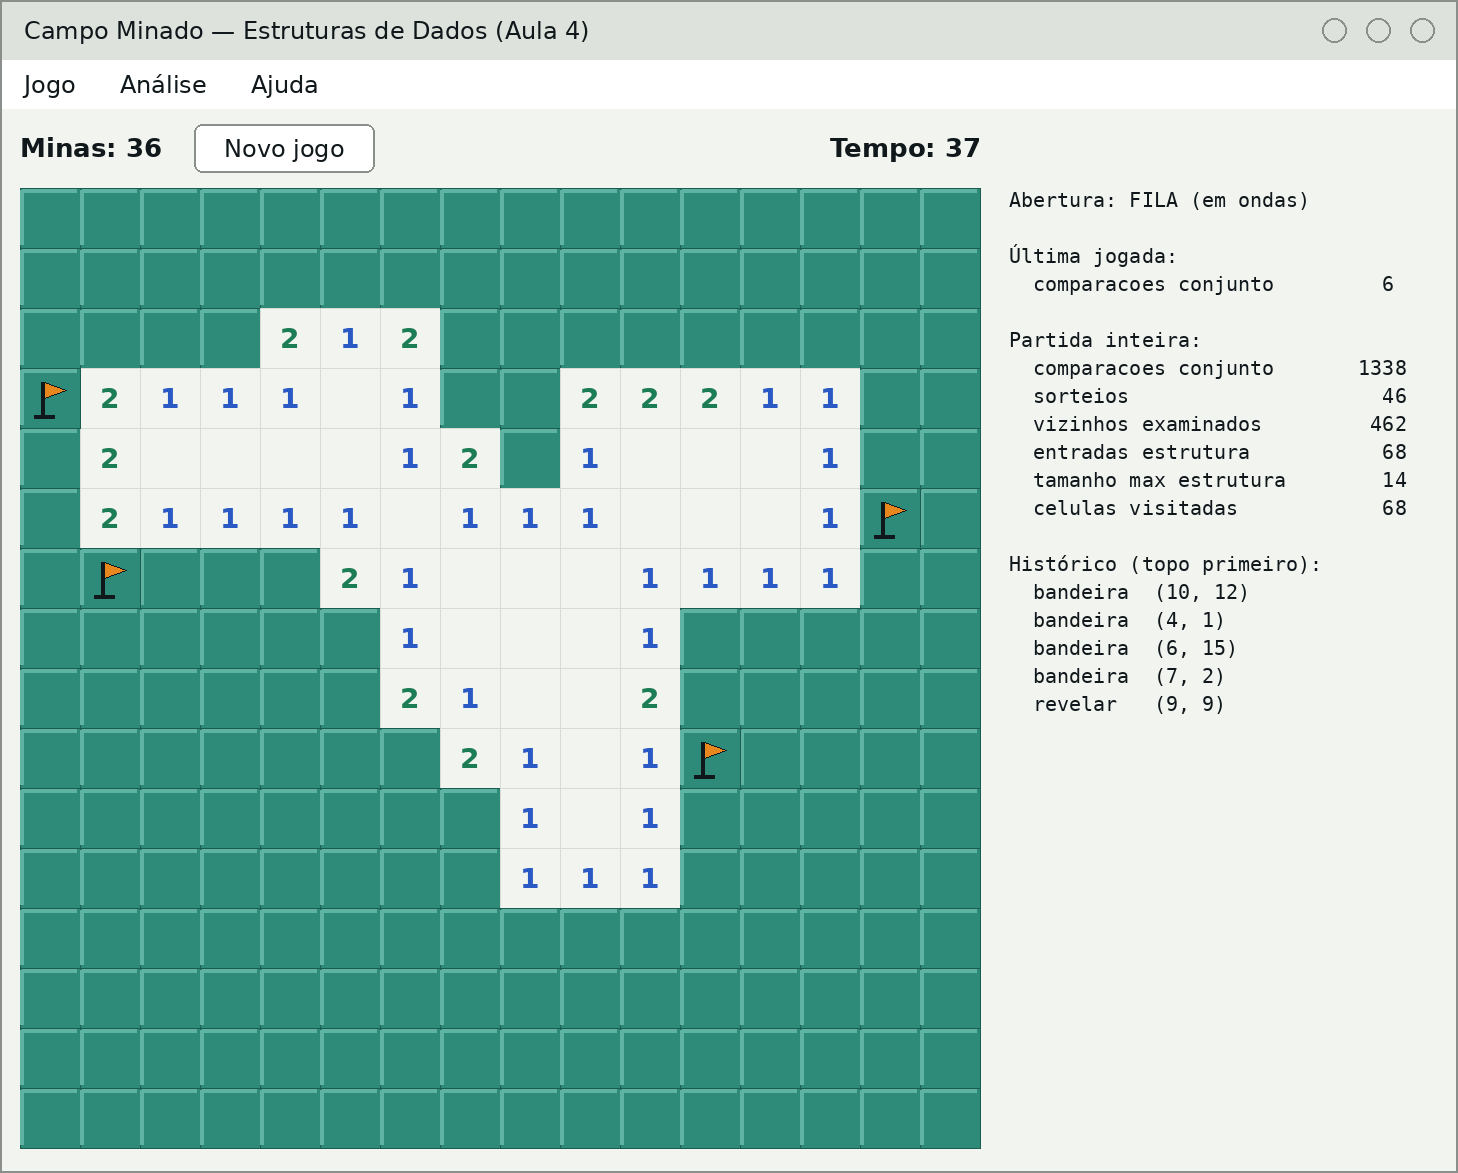
\includegraphics[width=0.78\textwidth]{figuras/janela_campo_minado.png}
  \caption{A interface gráfica, com o painel de análise (ilustração gerada a partir do código de
  desenho do jogo).}
\end{figure}

\section{A organização do programa}

A decisão de projeto mais importante é \textbf{separar a lógica da interface}. Todas as regras
ficam na classe \codigo{Tabuleiro}, que não imprime nada nem abre janelas. As interfaces só
chamam os métodos dela e desenham o resultado.

\begin{figure}[!htb]
\centering
\begin{tikzpicture}[caixa/.style={draw=edteal, fill=edtealclaro, line width=1pt, rounded corners=2pt,
    minimum width=3.1cm, minimum height=0.9cm, font=\small, align=center},
    seta/.style={-{Latex}, line width=1pt, edverde}]
  \node[caixa] (e) at (0,0) {\texttt{estruturas.py}\\Pilha, Fila, Conjunto};
  \node[caixa, fill=edlaranjaclaro, draw=edlaranja] (t) at (0,-1.7) {\texttt{tabuleiro.py}\\regras do jogo};
  \node[caixa] (r) at (4.4,-1.7) {\texttt{ranking.py}\\melhores tempos};
  \node[caixa] (gui) at (-4.4,-3.5) {\texttt{jogo\_gui.py}\\janela (tkinter)};
  \node[caixa] (ter) at (-1.2,-3.5) {\texttt{jogo\_terminal.py}\\texto};
  \node[caixa] (tes) at (2.0,-3.5) {\texttt{testes.py}\\testes automáticos};
  \node[caixa] (an) at (5.2,-3.5) {\texttt{analise\_...py}\\medições};
  \draw[seta] (e) -- (t);
  \foreach \x in {gui, ter, tes, an} \draw[seta] (\x.north) -- (t.south);
  \draw[seta] (gui.north) to[bend left=35] (r.north west);
  \draw[seta] (ter.north) -- (r.south west);
\end{tikzpicture}
\caption{Quem usa quem: as setas apontam para o módulo usado. As regras ficam num único lugar.}
\end{figure}

Vantagens: a mesma lógica serve às duas interfaces; os testes verificam as regras sem abrir
janela nenhuma; e dá para trocar a interface sem mexer nas regras (e vice-versa).

\section{Técnica 1: o tabuleiro numa lista linear}

Um tabuleiro parece pedir uma matriz, mas a solução guarda tudo em \textbf{listas lineares}, com
uma posição por célula — a lista contígua da Aula 1. A célula (linha, coluna) fica na posição
\[
\text{índice} = \text{linha} \times C + \text{coluna} \qquad \text{(contando a partir de 0)}.
\]

\begin{figure}[!htb]
\centering
\begin{tikzpicture}[scale=0.62]
  \foreach \l in {0,1,2} \foreach \c in {0,...,3} {
    \pgfmathtruncatemacro{\idx}{\l*4+\c}
    \draw[fill=edtealclaro, draw=edteal, line width=0.8pt] (\c, -\l) rectangle ++(0.95,0.95);
    \node[font=\small] at (\c+0.47, -\l+0.47) {\idx};
  }
  \node[font=\small, color=edcinza] at (1.9, 1.4) {tabuleiro 3 × 4};
  \foreach \i/\cor in {0/edtealclaro, 1/edtealclaro, 2/edtealclaro, 3/edtealclaro,
                      4/edlaranjaclaro, 5/edlaranjaclaro, 6/edlaranjaclaro, 7/edlaranjaclaro,
                      8/edfundo2, 9/edfundo2, 10/edfundo2, 11/edfundo2} {
    \draw[fill=\cor, draw=edteal, line width=0.8pt] (6.2+\i*0.95, -0.9) rectangle ++(0.9,0.9);
    \node[font=\small] at (6.2+\i*0.95+0.45, -0.45) {\i};
  }
  \node[font=\small, color=edcinza] at (11.9, 0.55) {a mesma coisa, numa lista linear};
  \node[font=\footnotesize, color=edteal] at (7.9, -1.5) {linha 0};
  \node[font=\footnotesize, color=edlaranja] at (11.7, -1.5) {linha 1};
  \node[font=\footnotesize, color=edverde] at (15.5, -1.5) {linha 2};
\end{tikzpicture}
\caption{Com 4 colunas, a célula (1,\,2) fica no índice $1 \times 4 + 2 = 6$.}
\end{figure}

\begin{lstlisting}
def indice(self, linha, coluna):
    return linha * self.colunas + coluna                  # O(1)

def coordenadas(self, indice):
    return indice // self.colunas, indice % self.colunas  # O(1)
\end{lstlisting}

Ler ou alterar qualquer célula custa $O(1)$. E um único número identifica cada célula, o que
simplifica guardar células em Conjuntos, Filas e Pilhas.

\section{Técnica 2: vizinhança e bordas}

As 8 direções ficam numa tupla de deslocamentos, sempre na mesma ordem. Para cada uma, calcula-se
a vizinha e descarta-se o que cair fora do tabuleiro:

\begin{lstlisting}
DIRECOES = ((-1, -1), (-1, 0), (-1, 1),     # noroeste, norte, nordeste
            (0, -1),           (0, 1),      # oeste, leste
            (1, -1),  (1, 0),  (1, 1))      # sudoeste, sul, sudeste

def vizinhos(self, indice):
    linha, coluna = self.coordenadas(indice)
    resultado = []
    for delta_linha, delta_coluna in DIRECOES:
        l, c = linha + delta_linha, coluna + delta_coluna
        if 0 <= l < self.linhas and 0 <= c < self.colunas:   # dentro do tabuleiro?
            resultado.append(self.indice(l, c))
    return resultado
\end{lstlisting}

São sempre 8 tentativas: custo $\Theta(1)$. A verificação de bordas é essencial. Sem ela, a
última célula de uma linha \enquote{enxergaria} a primeira célula da linha de baixo, porque na
lista linear elas são vizinhas de posição.

\section{Técnica 3: sortear minas sem repetição}

O sorteio usa o \textbf{Conjunto} da Aula 3, que já ignora valores repetidos:

\begin{lstlisting}
proibidas = Conjunto(self.contador)          # a célula clicada e suas vizinhas
proibidas.inserir(protegida)
for vizinha in self.vizinhos(protegida):
    proibidas.inserir(vizinha)

while self.minas.tamanho() < self.num_minas:
    candidata = self._gerador.randrange(self.total_celulas)
    if not proibidas.pertence(candidata):
        self.minas.inserir(candidata)        # o Conjunto ignora repetidas
\end{lstlisting}

Cada \codigo{inserir()} chama \codigo{pertence()}, que percorre as minas já sorteadas: $0 + 1 +
\dots + (k - 1) = \dfrac{k(k-1)}{2}$ comparações, ou seja, $O(k^2)$ — mais as tentativas
repetidas, que são poucas quando $k$ é pequeno perto do tabuleiro. No nível Difícil, foram 122
tentativas e 6.515 comparações.

\begin{aprofunde}
Uma alternativa sem repetições é o \textbf{embaralhamento de Fisher–Yates}: coloque numa lista os
índices permitidos e, de trás para a frente, troque cada posição com uma posição sorteada entre as
anteriores (inclusive ela). No fim, a lista está embaralhada com todas as ordens igualmente
prováveis, e as primeiras $k$ posições são as minas. Custo: $\Theta(L \cdot C)$, sem nenhuma
repetição. Vale mais a pena quando há muitas minas, caso em que o sorteio simples repetiria muito.
\end{aprofunde}

\section{Técnica 4: calcular os números percorrendo as minas}

A forma óbvia de calcular os números seria perguntar, para cada célula, \enquote{quantas das minhas
vizinhas são minas?}: $L \cdot C$ células, até 8 consultas ao Conjunto cada uma, e cada consulta
custando $O(k)$. Total: $O(L \cdot C \cdot k)$. A solução faz o contrário:

\begin{lstlisting}
for mina in self.minas.valores():            # só as k minas
    for vizinha in self.vizinhos(mina):      # até 8 vizinhas
        self.numeros[vizinha] += 1
\end{lstlisting}

São no máximo 8 passos por mina: $O(k)$. Medido com o \codigo{analise_complexidade.py}:

\begin{center}
\begin{tabularx}{\textwidth}{L C C C C}
\cab \tc{Nível} & \tcx{$L \times C$} & \tcx{$k$} & \tc{Percorrendo as minas} & \tc{Perguntando a cada célula} \\
Fácil & $9 \times 9$ & 10 & 65 & 5.110 \\
\rowcolor{edfundo} Médio & $16 \times 16$ & 40 & 294 & 68.664 \\
Difícil & $16 \times 30$ & 99 & 735 & 317.004 \\
\end{tabularx}
\end{center}

No nível Difícil, a forma ingênua faz cerca de \textbf{431 vezes} mais trabalho para chegar ao
mesmo resultado. Mudar o ponto de vista do algoritmo mudou a família do custo.

\section{Técnica 5: a abertura em cascata com Fila ou Pilha}

A abertura em cascata é um algoritmo clássico de \enquote{preenchimento de região}
(\emph{flood fill}). Ele mantém uma estrutura de células \textbf{pendentes}: retira uma, e, se ela
for 0, coloca na estrutura as vizinhas ainda fechadas.

\begin{lstlisting}
usar_fila = self.estrategia == "fila"
pendentes = Fila() if usar_fila else Pilha(self.total_celulas)
colocar = pendentes.enfileirar if usar_fila else pendentes.empilhar
retirar = pendentes.desenfileirar if usar_fila else pendentes.desempilhar

ordem = []
self._marcar_revelada(inicio)                # marca AO COLOCAR na estrutura
colocar(inicio)
while not pendentes.esta_vazia():
    atual = retirar()
    ordem.append(atual)
    if self.numeros[atual] != 0:
        continue                             # numerada: abre, mas não espalha
    for vizinha in self.vizinhos(atual):
        if not self.reveladas[vizinha] and not self.bandeiras.pertence(vizinha):
            self._marcar_revelada(vizinha)
            colocar(vizinha)
return ordem
\end{lstlisting}

Três detalhes fazem toda a diferença:

\begin{itemize}
  \item \textbf{Funções como valores:} \codigo{colocar} e \codigo{retirar} guardam as operações da
        estrutura escolhida, e o resto do algoritmo é o mesmo para Fila e Pilha.
  \item \textbf{Marcar ao colocar:} a célula é marcada como aberta no momento em que entra na
        estrutura. Assim, cada célula entra no máximo uma vez, e a abertura custa $O(L \cdot C)$.
        Se marcássemos só ao retirar, uma célula poderia entrar uma vez para cada vizinha que a
        visse antes de ela sair:
\end{itemize}

\begin{center}
\begin{tabularx}{0.85\textwidth}{C C C C}
\cab \tcx{$N$} & \tcx{Células ($N^2$)} & \tc{Entradas, marcando ao colocar} & \tc{Entradas, marcando ao retirar} \\
10 & 100 & 100 & 343 \\
\rowcolor{edfundo} 20 & 400 & 400 & 1.483 \\
40 & 1.600 & 1.600 & 6.163 \\
\end{tabularx}
\end{center}
{\small Tabuleiro $N \times N$ sem minas, aberto a partir do canto: o pior caso da cascata.}

\begin{itemize}
  \item \textbf{Fila ou Pilha:} as duas abrem exatamente as mesmas células, com o mesmo custo de
        tempo. Muda a \textbf{ordem}: a Fila abre em ondas a partir do clique (busca em largura);
        a Pilha segue um caminho em profundidade antes de voltar (busca em profundidade).
\end{itemize}

\begin{figure}[!htb]
  \centering
  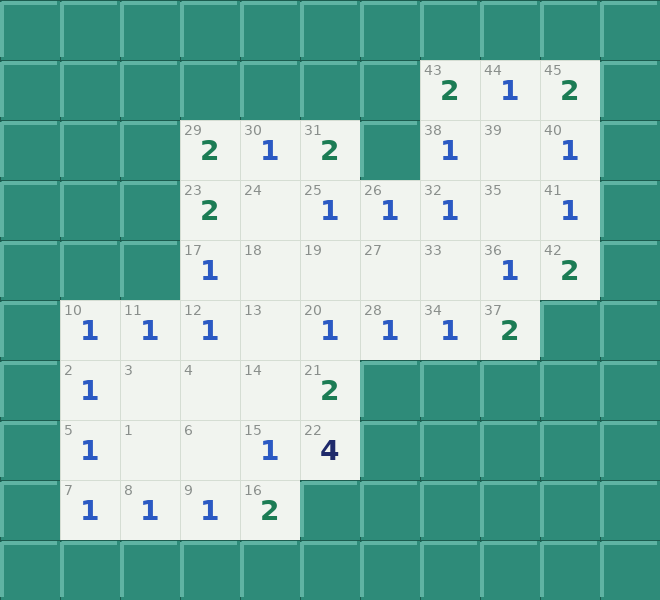
\includegraphics[width=0.45\textwidth]{figuras/ordem_fila.png}\hfill
  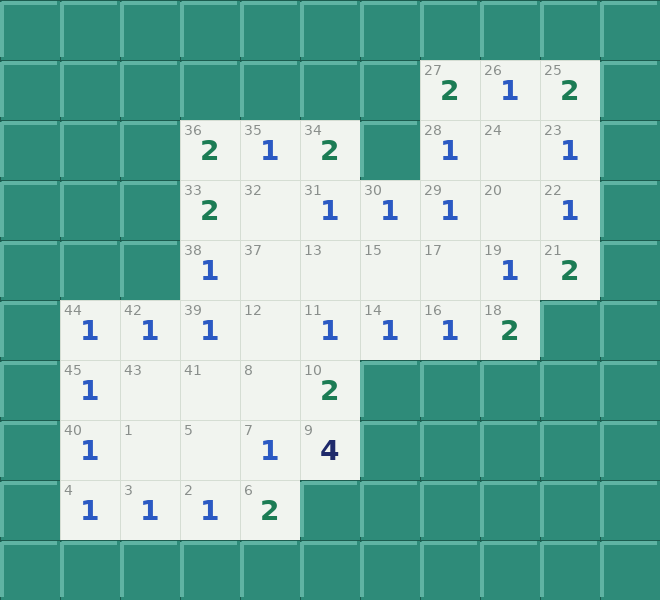
\includegraphics[width=0.45\textwidth]{figuras/ordem_pilha.png}
  \caption{Mesmo tabuleiro, mesmo clique: com Fila (esquerda) e com Pilha (direita). Os números
  pequenos indicam a ordem de abertura.}
\end{figure}

A diferença aparece na \textbf{memória}: a Fila guarda só a \enquote{frente da onda}; a Pilha pode
acumular muito mais células ao mesmo tempo. Por isso a Pilha contígua (de capacidade fixa, como
na Aula 2) é criada com capacidade $L \cdot C$.

\begin{center}
\begin{tabularx}{0.85\textwidth}{C C C C}
\cab \tcx{$N$} & \tc{Células} & \tc{Maior tamanho da Fila} & \tc{Maior tamanho da Pilha} \\
10 & 100 & 19 & 44 \\
\rowcolor{edfundo} 20 & 400 & 39 & 142 \\
40 & 1.600 & 79 & 487 \\
\rowcolor{edfundo} 80 & 6.400 & 159 & 1.777 \\
\end{tabularx}
\end{center}

\section{Técnica 6: vitória em \texorpdfstring{$O(1)$}{O(1)}}

Para saber se o jogador venceu, poderíamos varrer a lista \codigo{reveladas} a cada jogada:
$O(L \cdot C)$ por jogada. A solução mantém um contador, \codigo{celulas_seguras_restantes}, que
começa em $L \cdot C - k$ e diminui 1 a cada célula aberta. A vitória é simplesmente
\codigo{celulas_seguras_restantes == 0}: $O(1)$. É a mesma ideia do \codigo{tamanho} guardado na
Lista da Aula 1: \textbf{manter uma informação atualizada custa pouco e evita recalcular tudo}.

\section{Técnica 7: histórico com Pilha e o desfazer}

Cada jogada é empilhada como uma tupla \codigo{("revelar", linha, coluna)} ou
\codigo{("bandeira", linha, coluna)}. Desfazer consulta o \textbf{topo}: se for uma bandeira,
desempilha e desfaz; se for um \enquote{revelar}, não faz nada, porque abrir uma célula não tem volta.

\begin{lstlisting}
acao, linha, coluna = self.historico.consultar_topo()
if acao != "bandeira":
    return None                              # revelar não tem volta
self.historico.desempilhar()
\end{lstlisting}

É o comportamento LIFO em ação: só o último elemento é acessível. As \enquote{últimas jogadas}
mostradas no painel são os valores da Pilha do topo para a base, sem remover nada.

\section{Técnica 8: ranking com inserção ordenada}

O ranking guarda os 10 melhores tempos de cada nível numa lista sempre ordenada. Para inserir um
recorde, faz um passo do Insertion Sort: coloca no fim e desloca para a direita os tempos maiores.
Custo $O(n)$ no pior caso e $O(1)$ no melhor. Ao carregar o arquivo, ordena com o Insertion Sort
completo — e, como o próprio programa salva o arquivo já ordenado, cai no \textbf{melhor caso},
$\Theta(n)$, exatamente o cenário do capítulo 9.

\section{Técnica 9: medir contando operações}

A classe \codigo{ContadorOperacoes} registra, por categoria, o trabalho de cada jogada:
\enquote{entradas na estrutura}, \enquote{células visitadas}, \enquote{vizinhos examinados},
\enquote{comparações no Conjunto}. O próprio \codigo{pertence()} do Conjunto conta cada
comparação que faz — por isso ele usa um laço explícito em vez de \codigo{valor in lista}, que
esconderia o trabalho. É a contagem de operações do capítulo 2, aplicada a um programa inteiro.

\section{Técnica 10: interfaces, eventos e testes}

\begin{itemize}
  \item \textbf{Programação orientada a eventos:} a interface gráfica não tem um laço que lê
        comandos. Ela registra funções que o tkinter chama quando algo acontece
        (\codigo{canvas.bind("<Button-1>", ...)} para o clique) e usa \codigo{raiz.after(ms, funcao)}
        para agendar ações no futuro: o relógio e cada quadro da animação da abertura.
  \item \textbf{Desenho com etiquetas:} cada célula desenhada no Canvas recebe a etiqueta
        \codigo{"c<indice>"}, para ser apagada e redesenhada sozinha, sem redesenhar o tabuleiro todo.
  \item \textbf{Testes com semente fixa:} com \codigo{random.Random(semente)}, o sorteio é sempre o
        mesmo, e os testes podem conferir resultados exatos. O \codigo{testes.py} usa o tabuleiro da
        Parte A e confere, por exemplo, a ordem exata de abertura com Fila e com Pilha.
\end{itemize}

\section{Resumo dos custos}

\begin{center}
\begin{tabularx}{\textwidth}{L C L}
\cab \tc{Operação} & \tc{Custo} & \tc{Técnica} \\
\codigo{indice()}, \codigo{coordenadas()}, \codigo{vizinhos()} & $\Theta(1)$ & lista linear, 8 direções \\
\rowcolor{edfundo} sortear as minas & $O(k^2)$ & Conjunto sobre lista \\
calcular os números & $O(k)$ & percorrer as minas \\
\rowcolor{edfundo} abertura em cascata & $O(L \cdot C \cdot f)$ & Fila ou Pilha, marcar ao colocar \\
verificar vitória & $\Theta(1)$ & contador de células seguras \\
\rowcolor{edfundo} bandeira, desfazer & $O(f)$ & Conjunto e Pilha \\
registrar recorde & $O(n)$ & inserção ordenada \\
\end{tabularx}
\end{center}
{\small $f$ = número de bandeiras. Na abertura, cada vizinha examinada consulta o Conjunto de
bandeiras ($O(f)$); com uma lista de booleanos, essa consulta seria $O(1)$ e a abertura,
$O(L \cdot C)$.}

\begin{exrapido}
No tabuleiro 5 × 5 da Parte A (5 colunas, contando a partir de 0 no código): (a) qual é o índice
da célula (3,\,4)? (b) quais são os índices das vizinhas da célula de índice 0? (c) quantas
vizinhas tem a célula de índice 12?
\end{exrapido}

\begin{respostas}
  \resp{14.1} (a) $3 \times 5 + 4 = 19$ — é a mina da linha 4, coluna 5 (contando a partir de 1).
  (b) A célula 0 é o canto superior esquerdo: vizinhas 1, 5 e 6. (c) A célula 12 é
  (2,\,2), no meio do tabuleiro: 8 vizinhas.
\end{respostas}
